\makeatletter % Use \makeatletter to make '@' a letter
\def\input@path{{../}} % Define input path to parent directory
\makeatother % Restore default category code of '@'

\documentclass[../main.tex]{subfiles}

\begin{document}

\chapter{Introduction}\label{ch:introduction}

In this thesis, we focus on a specific aspect of theoretical high-energy physics: the resummation of the Thrust event-shape distribution in electron-positron ($e^+e^-$) collisions.

\begin{figure}[h!]
    \centering
    \begin{tikzpicture}
    \begin{feynman}
        \vertex (a);
        \vertex [above left=of a] (i1) {$e^{-}$};
        \vertex [below left=of a] (i2) {$e^{+}$};
        \vertex (b) [right=of a];
        \vertex [above right=of b] (f1) {$q$};
        \vertex [below right=of b] (f2) {$\bar{q}$};

        \diagram* {
            (i1) -- [fermion] (a) -- [fermion] (i2),
            (a) -- [photon, edge label=\(\gamma^*\), momentum'=\(k\)] (b),
            (f2) -- [fermion] (b) -- [fermion] (f1),
        };

    \end{feynman}
\end{tikzpicture}
    \caption{Tree-level Feynman diagram of electron-positron annihilation producing a virtual photon that decays into a quark-antiquark pair.}
    \label{fig:ep_annihilation}
\end{figure}


Electron-positron annihilation has been extensively studied, particularly during the operation of LEP (Large Electron-Positron Collider) at CERN from 1989 to 2000. 
It provides an optimal environment for precision studies in high-energy physics. 
Unlike hadron colliders, which are complicated by strongly interacting initial states, LEP has provided extremely accurate measurements of Standard Model quantities such as the Z-boson mass. 
These results tightly constrain beyond-the-Standard Model physics. Precision data from LEP is also used in Quantum Chromodynamics (QCD) studies, for example, to determine the strong coupling constant, $\alpha_S$.

As is typical in physics, the equations governing these interactions are highly complex, finding exact solutions is nearly impossible.
Therefore, functions of interest are often expanded perturbatively, meaning they are expressed as a power series in a small parameter.

For the electromagnetic interaction, this small parameter is the fine structure constant (or electromagnetic coupling constant) $\alpha_{em} \sim \frac{1}{137}$.

For interactions involving the strong force, it is natural to use the strong coupling constant, $\alpha_S$.

Extraction of $\alpha_S$ can be done from event shape variables such as the thrust.


\section{Thrust variable}\label{sec:Thrust}

Thrust $T$ is defined as:

\begin{equation} \label{eq:Thrust}
    T = \max_{\vec{n}} \frac{\sum_i |\vec{p}_i \cdot \vec{n}|}{\sum_i |\vec{p}_i|} \stackrel{\text{def}}{=} 1-\tau
\end{equation}

where the sum is over all final state particles and $\vec{n}$ is a unit vector.
In practice, the sum may be carried over the detected particles only. 
The thrust distribution represents the probability of observing a given value of $T$ in $e^+e^-$ annihilation,\emph{i.e} the probability of observing a given configuration of momenta of final-state particles 
with respect to the thrust axis.  

It can be seen from this definition that the thrust is an infrared and collinear safe quantity, that is, it is insensitive to the emission of zero momentum particles and to the splitting of 
one particle into two collinear ones.

In fact, contribution from soft particles with $\vec{p_i}\to 0$ drop out, and collinear splitting does not change the thrust:
$\vert (1-\lambda)\vec{p_i}\cdot \vec{n} \vert + \vert \lambda \vec{p_i}\cdot \vec{n}\vert = \vert \vec{p_i}\cdot \vec{n} \vert$ and 
$\vert (1-\lambda)\vec{p_i} \vert + \vert \lambda \vec{p_i}\vert = \vert \vec{p_i} \vert$

Formally, infrared-safe observables are the one which do not distinguish between (n+1) partons and n partons in the soft/collinear limit, \emph{i.e},
are insensitive to what happens at long-distance.

Infrared safe observables are important in the context of perturbative QCD, because they allow for a meaningful comparison between theory and experiment. 

One difficulty in achieving an accurate theoretical prediction from QCD has been the complexity of the relevant fixed-order calculations. Indeed, while the next-to-leading-order (NLO) results 
for event shapes have been known since 1980 \cite{Ellis:1980wv}, the relevant next-to-next-leading order (NNLO) calculations were completed only in 2007 \cite{Gehrmann-DeRidder:2007nzq}.

\begin{figure}[h]
    \centering
    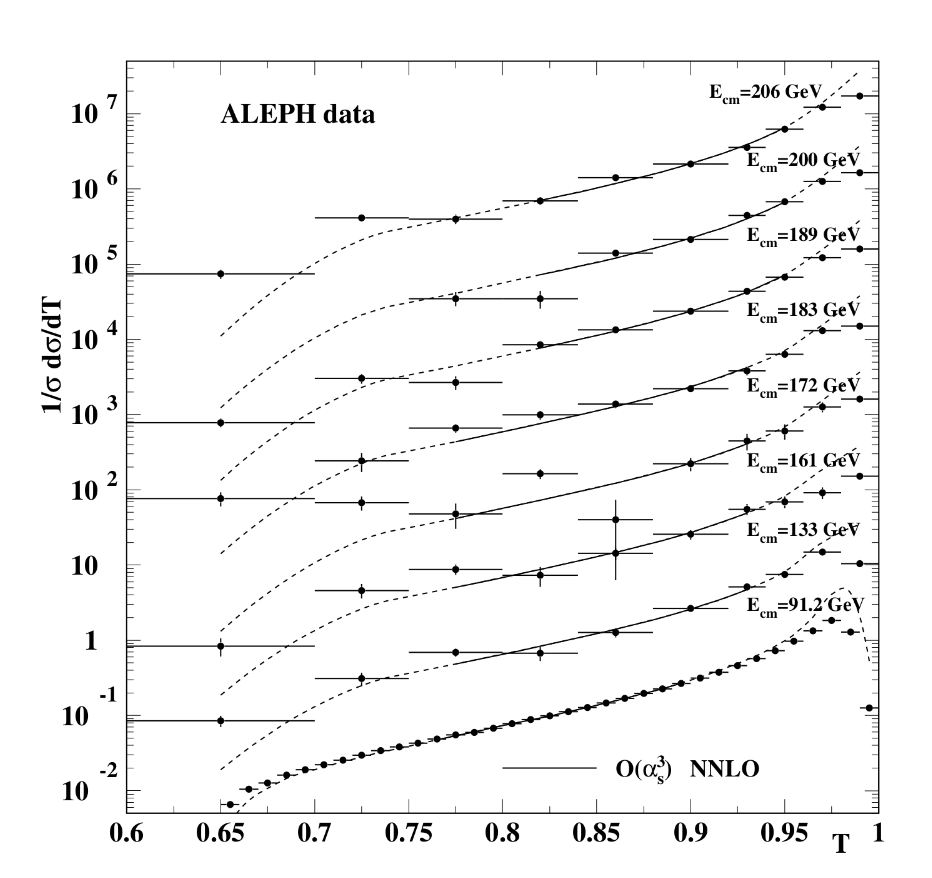
\includegraphics[width=0.5\textwidth]{figures/LEP_Thrust_NNLO.png}
    \caption{Distributions measured by ALEPH, after correction for backgrounds and detector
    effects of thrust at energies between 91.2 and 206
    GeV together with the fitted NNLO QCD predictions. The error bars correspond to statistical
    uncertainties.The plotted
    distributions are scaled by arbitrary factors for presentation. Image taken from \cite{Dissertori_2008}.}
    \label{fig:LEP_Thrust_NNLO}
\end{figure}

We can see from \cref{fig:LEP_Thrust_NNLO} that the NNLO calculation is in good agreement with the data, except for the region near $T=0.5$ (spherical final state) and $T=1$ (pencil-like final state).

The thrust distribution for $T\simeq 1$ is dominated by two-jet configurations, \emph{i.e.} the final state particles are mainly two partons emitted back-to-back like \cref{fig:ep_annihilation}, while 
the tail of the distribution near $T= 0.5$ is dominated by multijet final states.


\subsection{Thrust distribution} \label{subsec:Thrust_distribution}

The cross section is defined as the probability of observing a final state with a given thrust value $\tau$:

\begin{equation}\label{eq:cross_section}
    \sigma(\tau) = \int^\tau_0 \dd{\tau'} \dv{\sigma}{\tau'}
\end{equation}

It can be seen that a two-particle final state has fixed $T = 1$, in fact at the zeroth order of the fixed order \cref{eq:LO fixed order} it's 
a delta distribution, consequently the thrust distribution receives its first non-trivial contribution from three-particle final states.

The lower limit on $T$ depends on the number of final-state particles.
Neglecting masses, $T_{min} = 2/3$ for three particles, corresponding to a symmetric
configuration. For four particles the minimum thrust corresponds to final-state
momenta forming the vertices of a regular tetrahedron, each making an angle
$\cos^{-1}(1/\sqrt{3})$ with respect to the thrust axis. Thus $T_{min} = 1/\sqrt{3} = 0.577$ in this
case . For more than four particles, $T_{min}$ approaches $1/2$ from above as the number of particles increases.

At large values o f $T$, however, there are terms in higher order that become enhanced by powers o f $\ln(1 - T)$.
In this kinematical region the real expansion parameter is the
large effective coupling $\alpha_s \ln^2(\tau)$ and therefore
any finite-order perturbative calculation cannot give an accurate evaluation o f the cross section.

For example, at leading order in perturbation theory the thrust distribution has the form:

\begin{equation}\label{eq:LO fixed order}
    \frac{1}{\sigma_0}\dv{\sigma}{\tau} = \delta(\tau) + \frac{2\alpha_s}{3\pi} \qty[\frac{-4 \ln \tau - 3}{\tau} + \dots]
\end{equation}

where $\sigma_0$ is the born cross section and the ellipsis denotes terms that are regular as $\tau \to 0$. 
Upon integration over $\tau$, we obtain the cumulative distribution:

\begin{equation}
    R(\tau) = \int_0^\tau \dd{\tau'} \frac{1}{\sigma_0}\dv{\sigma}{\tau'} = 1 + \frac{2\alpha_s}{3\pi} \qty[-2 \ln^2 \tau - 3 \ln \tau + \dots] 
\end{equation}

Double logarithmic terms of the form $\alpha_s^n \ln^{2n}\tau$ plagues the fixed order expansion in the strong coupling. In the dijet region, higher order 
terms are as important as lower order ones and resummation is needed to obtain a reliable prediction.


\subsection{Fixed Order Cross Section}

The fixed-order thrust distribution has been calculated to leading order analytically and
to NLO and NNLO numerically. At a centre-of-mass energy $Q$ and for a renormalization scale $\mu$ takes the form:

\begin{equation}\label{eq:Fixed_order}
    \frac{1}{\sigma_0} \dv{\sigma}{\tau} \qty(\tau,Q) = \delta(\tau) + \frac{\alpha_s(\mu)}{2\pi}\dv{A}{\tau} \qty(\tau) + \qty(\frac{\alpha_s(\mu)}{2\pi})^2 \dv{B}{\tau} \qty(\tau,\frac{\mu}{Q}) + \qty(\frac{\alpha_s(\mu)}{2\pi})^3 \dv{C}{\tau} \qty(\tau,\frac{\mu}{Q}) + \order{\alpha_s^4}
\end{equation}

where the complete leading order expression for the thrust distribution reads\cite{Ellis:1980wv}:

\begin{equation}\label{eq:Fixed_order_A}
    \dv{A}{\tau}(\tau) =  \text{C}_F \left(9 \tau -\frac{3}{\tau }+\left(-6 +\frac{4}{(1-\tau ) \tau }\right) \log \left(\frac{1-2 \tau }{\tau }\right)+6\right)
\end{equation}

As said above, this expansion breaks down near the dijet limit $\tau \to 0$ due to the presence of large logarithms and 
we need to resum these terms to all orders in $\alpha_s$ to obtain a reliable prediction.

For later convenience we consider also the integrated distribution or cumulant distribution:

\begin{equation}
    R(\tau) = \int_0^\tau \dd{\tau'} \frac{1}{\sigma}\dv{\sigma}{\tau'} 
\end{equation}

which has the following fixed-order expansion:

\begin{equation}\label{eq:Fixed_order_R}
    R(\tau) = 1 + A(\tau) \frac{\alpha_s(\mu)}{2\pi} + B(\tau,\mu) \frac{\alpha_s(\mu)}{2\pi}^2 + C(\tau,\mu)\frac{\alpha_s(\mu)}{2\pi}^3 + \order{\alpha_s^4}
\end{equation}

\end{document}